\chapter{Gestión de residuos sólidos}
\label{chap2}
\ifpdf
  \graphicspath{{Chapter2/Chapter2Figs/}}
\else
  \graphicspath{{Chapter2/Chapter2Figs/}}\fi

\markboth{\hfill \thechapter. Gestión de residuos sólidos}{\hfill \thechapter. Gestión de residuos sólidos}

Se conoce como residuo a cualquier material en estado sólido, líquido o gaseoso resultante de los procesos de producción, transformación y utilización, que carente de valor para su propietario, éste decide abandonarlo.
%Agregar estadistica de genearacion diaria de residuos por personas de la ciudad de Asuncion

El decreto N\grad 7391, del 28 de junio de 2017, que reglamenta la Ley N\grad 3956/2009, acerca de la ``Gestión Integral de los Residuos Sólidos en la República del Paraguay", clasifica los residuos en:

\begin{itemize}
\item \textbf{Residuos sólidos urbanos:} Los generados en cada habitación, unidad habitacional o similares que resultan de la eliminación de los materiales que se utilizan en las actividades domésticas, de los productos que se consumen y de sus envases, embalajes o empaques, y los provenientes de cualquier otra actividad que genere residuos sólidos con características domiciliarias y los resultantes de la limpieza de las vías públicas y áreas comunes.
\item \textbf{Residuos de manejo especial:} Los generados en los procesos productivos que no reúnen las características para ser considerados como peligrosos o como residuos sólidos urbanos, o que son producidos por grandes generadores de residuos sólidos urbanos. Entre ellos se encuentran los provenientes de servicios de la salud, aquellos generados en los procesos productivos e instalaciones industriales y comerciales, también los generados por la actividades agrícolas, pesqueras y forestales, los de servicios de transportes, resultantes de las actividades que se realizan en terminales de transportes; también se incluyen los residuos de la construcción civil, los tecnológicos, los provenientes del tratamiento de aguas residuales, los neumáticos usados, muebles, los residuos de minería e hidrocarburos.
\item \textbf{Residuos peligrosos:} Resultantes de los procesos industriales y productos que han sido adquiridos y/o desechados, y que por sus características explosivas, inflamables, oxidantes, tóxicas, infecciosas, radioactivas, corrosivas, etc, pueden causar riesgos presentes o futuros a la calidad de vida de las personas o afectar el suelo, la flora, la fauna, contaminar el aire o las aguas de manera tal que dañen la salud humana o ambiental del país.
\end{itemize}

\section{Procesos de la gestión de residuos sólidos}

La gestión de residuos sólidos o SWM implica varios procesos que pueden dar lugar a problemas relacionados con áreas como la organización, el control, la logística, la planificación y el reciclaje. Es una actividad multidisciplinaria que contiene decisiones de criterios múltiples en cada etapa de su ciclo de vida. 

La gestión integral de residuos sólidos es el conjunto de acciones que se aplican en el manejo de los desechos desde su generación hasta su disposición final, basándose en criterios sanitarios, ambientales y de viabilidad técnica y económica para la reducción en la fuente de aprovechamiento, tratamiento y disposición final.

% Existen investigaciones en varios aspectos, como el área de pronóstico de generación de residuos, el monitoreo de los sistemas de recolección de contenedores, la gestión del transporte de contenedores y la predicción de la instalación de nuevas plantas de eliminación de residuos.

En el trabajo de \citet{VitorinodeSouzaMelare2017TechnologiesReview} se agrupan los procesos de SWM en seis categorías:
\begin{itemize}
\item Gestión de recogida, recorrido y transporte; 
\item Gestión y seguimiento de contenedores; 
\item Reciclaje de residuos sólidos y gestión de residuos electrónicos;
\item Administración pública y desarrollo sostenible; 
\item Métodos de previsión y planificación; y 
\item Determinación de sitios de disposición de residuos.
\end{itemize}

\subsection{La gestión de recogida, recorrido y transporte}
La recogida de los residuos consiste en su recolección para trasladarlos a su disposición final. Se distinguen dos tipos de recogida: selectiva y no selectiva.

La recogida selectiva consiste en agrupar y clasificar los residuos según sus características y propiedades con el fin de facilitar su tratamiento, en este tipo de recogida la ciudadanía tiene un rol esencial. En la recogida no selectiva los residuos se depositan en los contenedores y/o cestos de basuras sin ningún tipo de separación.

El transporte es la acción de trasladar los residuos sólidos de una fase de su gestión a otra, mientras que el recorrido se refiere al trayecto o camino que sigue el vehículo desde el inicio hasta el fin de sus actividades. Hay que tener en cuenta el problema que se asocia con el movimiento diario de los vehículos, este incide directamente sobre las calles, que deben estar adecuadamente acondicionadas, también en muchos casos es fuente de molestias para los vecinos debido a los malos olores, ruidos, tráfico, contaminación, entre otros.

\subsection{Gestión y seguimiento de contenedores}

Se pueden detectar dos escenarios: (1) áreas críticas con contenedores que siempre están llenos, que deben ser reemplazados con contenedores de mayor capacidad; o (2) áreas cuyos contenedores están siempre vacíos. Los costos destinados en el mantenimiento de los vehículos de recolección y combustibles pueden ser reducidos mediante tecnologías que controlen el nivel del contenedor, desplazándose así el vehículo solo cuando los contenedores se encuentren en el nivel adecuado para la recolección \citep{VitorinodeSouzaMelare2017TechnologiesReview, Akhtar2017BacktrackingOptimization}.

En la Figura \ref{fig:contenedoresMDA} se observan los contenedores móviles que se encuentran distribuidos en el microcentro de la ciudad de Asunción y en la zona de su costanera.

\begin{figure}[H]
    \centering
    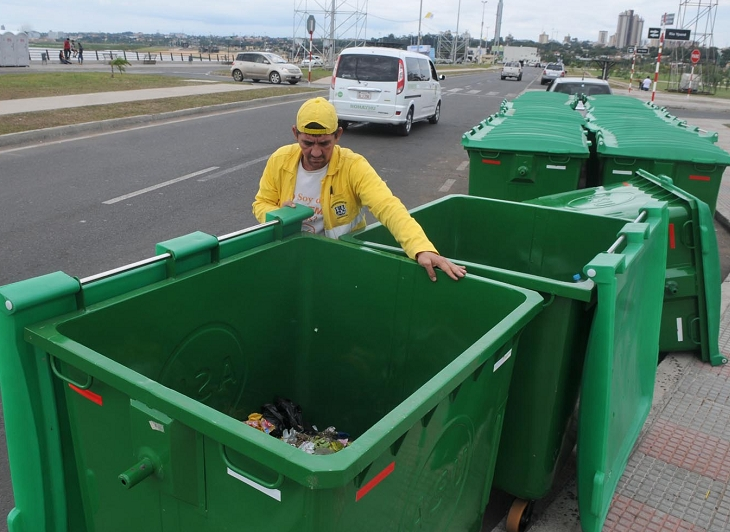
\includegraphics[width=7cm]{contenedores_mda.png}
    \caption{Contenedores de la ciudad de Asunción. [Fuente: Diario Última Hora (2015)]}
    \label{fig:contenedoresMDA}
\end{figure}

\subsection{Reciclaje de residuos sólidos}

El reciclaje es el resultado de una serie de actividades a través de las cuales, materiales que se tornarían residuos, son desviados, siendo recolectados, separados y procesados para ser usados como materia prima en la producción de un nuevo producto de composición semejante.

Entre los beneficios y ventajas del reciclaje se encuentran: la preservación de los recursos naturales, menor contaminación, ahorro de energía, dinero y petróleo, además, fomenta el consumo responsable y genera empleos.

\subsection{Administración pública y desarrollo sostenible}

La gestión de los residuos sólidos en el Paraguay, así como en la mayoría de los demás países, recae en el fuero municipal, se debe contar con políticas y estrategias nacionales para el desarrollo sostenible de la misma. La ausencia de planificación e infraestructura inadecuada para la eliminación de residuos sólidos conduce a una gran cantidad de residuos que se descargan en áreas públicas sin preparación del suelo, como vertederos a cielo abierto y ríos.

\subsection{Métodos de previsión y planificación}

El proceso de desarrollo urbano conlleva el crecimiento poblacional, cambios en patrones de consumo e incremento en el ingreso, siendo éstos, los principales factores que explican el aumento en la generación de residuos sólidos domiciliarios \citep{Vasquez2005ModeloChile}. Es por ello que es importante la elaboración de planes relacionados a la reducción de residuos sólidos, y la implementación de técnicas de previsión y modelos para predecir la generación de residuos, aumentando de esta manera la vida útil de los rellenos sanitarios en cuanto a su capacidad operativa o planes de expansión de instalaciones (tratamiento, traslado, y disposición).

\subsection{Determinación de sitios de disposición de residuos}

La selección de sitios para la disposición de residuos es un proceso complejo y considera criterios relacionados con el medio ambiente (suelo, características, declinación de la tierra, agua subterránea, ecosistema y geología), económico (presencia de caminos, distancia de las áreas residenciales, acceso al sitio y distancia de los centros de generación de residuos), y perspectivas sociales (aceptación de la población, proximidad a aeropuertos y sitios arqueológicos) \citep{Gbanie2013ModellingLeone}. Los métodos indiscriminados de eliminación de residuos han provocado la contaminación de cuerpos de agua, suelo y aire, lo que presenta importantes riesgos para la salud pública.

\section{Gestión de residuos sólidos urbanos en la ciudad de Asunción}

El área de estudio es Asunción, capital y ciudad más poblada de la República del Paraguay (según las proyecciones de \citet*{DireccionGeneraldeEstadistica2015Paraguay2000-2025} para el año 2019 se estima una población aproximada de 522.287 habitantes). Es un municipio autónomo administrado como Distrito capital, cuenta con una superficie de 117 km$^{2}$. El ingreso promedio de personas en ómnibus del transporte público y vehículos privados de los municipios aledaños es alrededor de 1.320.000 diariamente. Este análisis se hace en base a cálculos estimativos de la Unidad Coordinadora del Programa Metrobús del Ministerio de Obras Públicas y Comunicaciones (MOPC) \citep{DiarioABCColor2016PorColor}. La cantidad de personas que convergen diariamente en Asunción trae consigo una alta generación de residuos, y esto hace que la complejidad en la gestión sea cada vez mayor.

Para el desarrollo de esta investigación se trabaja estrechamente con la DSU de la MDA, entidad encargada de la regulación y prestación de servicios de aseo, recolección, disposición y tratamiento de los residuos del municipio, así como también del equipamiento, mantenimiento, limpieza y ornato de la infraestructura pública del municipio, incluyendo las calles, avenidas, parques, plazas, balnearios y demás lugares públicos.

% Según Rodrigo Velázquez, director de la DSU, el promedio diario normal de basura recogida suele ser entre 800.000 y 900.000 kilos \citep{LaNacion2016AsuncionBasura} [Dato obtenido en 9 de Enero de 2016]. 

En la actualidad, el Departamento de Recolección de la DSU es responsable de la recolección de residuos sólidos urbanos y divide la ciudad en 134 zonas para realizar la labor. Como mínimo, debe existir una calle empedrada para que los vehículos recolectores recojan los residuos, éste es el motivo por el que lugares marginales como los barrios denominados ``Bañados Norte y Sur'' no son beneficiados con el servicio.

% El municipio cuenta con contenedores distribuidos por el microcentro capitalino, estos son recogidos de la misma manera que los residuos domiciliarios.

\subsection{Procedimiento de recolección de residuos urbanos en la Municipalidad de Asunción}

% A continuación se detalla el procedimiento llevado a cabo habitualmente para la recolección de los residuos domiciliarios:
A continuación se detalla el procedimiento que se lleva a cabo habitualmente para la recolección de los residuos domiciliarios:

\begin{enumerate}
% \item Se establecen los días y frecuencias de recolección para cada zona.
\item Un equipo de trabajo que cuenta con un chofer y tres recolectores es asignado a un vehículo y una zona. El vehículo es identificado por su chapa o por el número de identificación del camión proveído por la DSU.
\item Se realiza una recogida no selectiva.
\item El vehículo recolector inicia su recorrido cuando parte de la DSU en dirección a su zona. Antes de partir se controla el nivel de combustible y de acuerdo a esto se procede a la carga del mismo, en caso de que fuese necesario. Se entrega al chofer una orden de trabajo del día con la hora de salida. En la Figura \ref{fig:vehiculoRecolectorMDA}, se muestran vehículos recolectores de la MDA.

\begin{figure}[H]
    \centering
    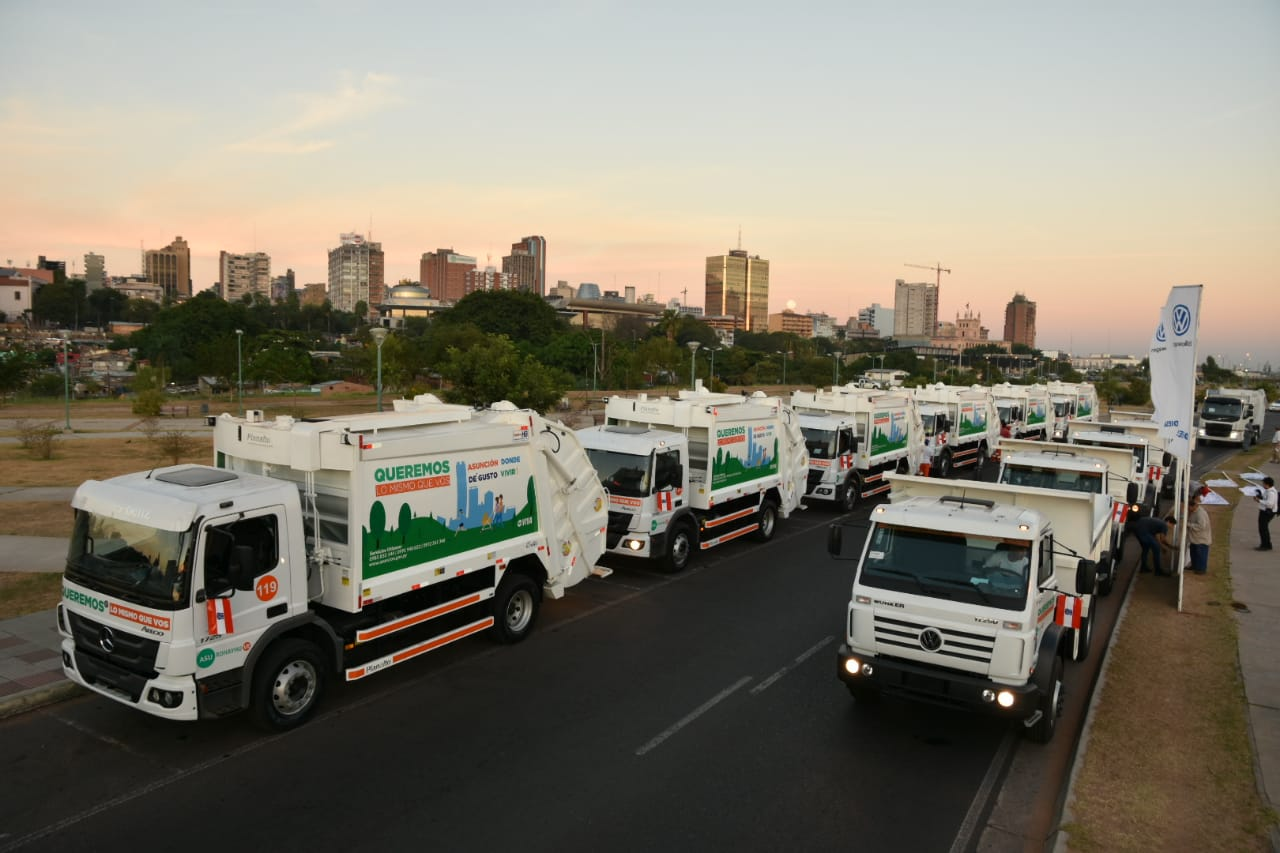
\includegraphics[width=7cm]{camion_recolector_mda.png}
    \caption{Vehículos recolectores de la MDA. [Fuente: MDA(2018)]}
    \label{fig:vehiculoRecolectorMDA}
\end{figure}

\item Luego de haber recogido toda la basura domiciliaria de la zona, el vehículo se dirige al relleno sanitario Cateura para depositar los residuos. 
\item Una vez que el chofer llega a Cateura, el camión pasa por un pesaje por ejes con báscula y el chofer entrega la orden de trabajo a un fiscalizador que se encuentra en el puesto de pesaje. Un grupo de personas de seguridad se encargan de coordinar la entrada y salida de vehículos, así como de guiar la descarga de lo recolectado. 
\item Una vez que se vacía el vehículo, uno de los encargados guía nuevamente al chofer hacia la salida, en donde el vehículo es pesado de vuelta, calculando el peso de lo recolectado resultado de la diferencia del peso de entrada y salida, que se detalla en la orden de trabajo la cual es devuelta al chofer. En la orden de trabajo también se especifican la hora de entrada y salida del vehículo al relleno sanitario.
\item El equipo vuelve al punto de partida una vez vaciado el vehículo recolector y el chofer entrega la orden de trabajo al Departamento de Recolección.  
\end{enumerate}

Generalmente, el vehículo tiene capacidad suficiente para realizar un solo viaje de su zona a Cateura, pero si no es el caso, debe realizar la cantidad de viajes necesarios hasta recolectar todos los residuos domiciliarios de la zona en cuestión. La carga máxima admitida de un vehículo recolector en circulación por el Departamento de Recolección de la DSU es de 8.500 kilogramos (kg). En caso de que el equipo de trabajo estime, en base a su experiencia, que la cantidad total a recoger de la zona será mayor a la permitida, entonces realizará más de un viaje a Cateura.

La segregación de los residuos no forma parte del proceso llevado a cabo por la DSU, es por ello que en Cateura se encuentran trabajando los gancheros, personas dedicadas a recuperar, separar o reducir, de los residuos sólidos urbanos, aquellos que posean valor comercial para su reutilización o reciclaje.

El servicio de recolección domiciliaria se realiza de lunes a sábados, y se divide en tres turnos: mañana, tarde y noche; donde cada turno tiene una duración máxima de 6 horas debido al carácter insalubre de las tareas realizadas por el personal encargado de brindar el servicio.

En la Figura \ref{fig:zonasRecoleccion} se muestran las zonas de recolección de basura de Asunción. Las zonas pintadas en celeste corresponden al microcentro de Asunción y tienen un tratamiento diferente a las demás, ya que son las únicas que son atendidas de lunes a viernes y sus residuos son recolectados en el turno noche debido al poco tráfico registrado en esas calles en comparación a cualquier otro turno. De igual manera, las avenidas más importantes de la ciudad también son recolectadas en el turno noche de lunes a viernes. Las demás zonas reciben el servicio cada dos días, tres veces por semana.

\begin{figure}[H]
    \centering
    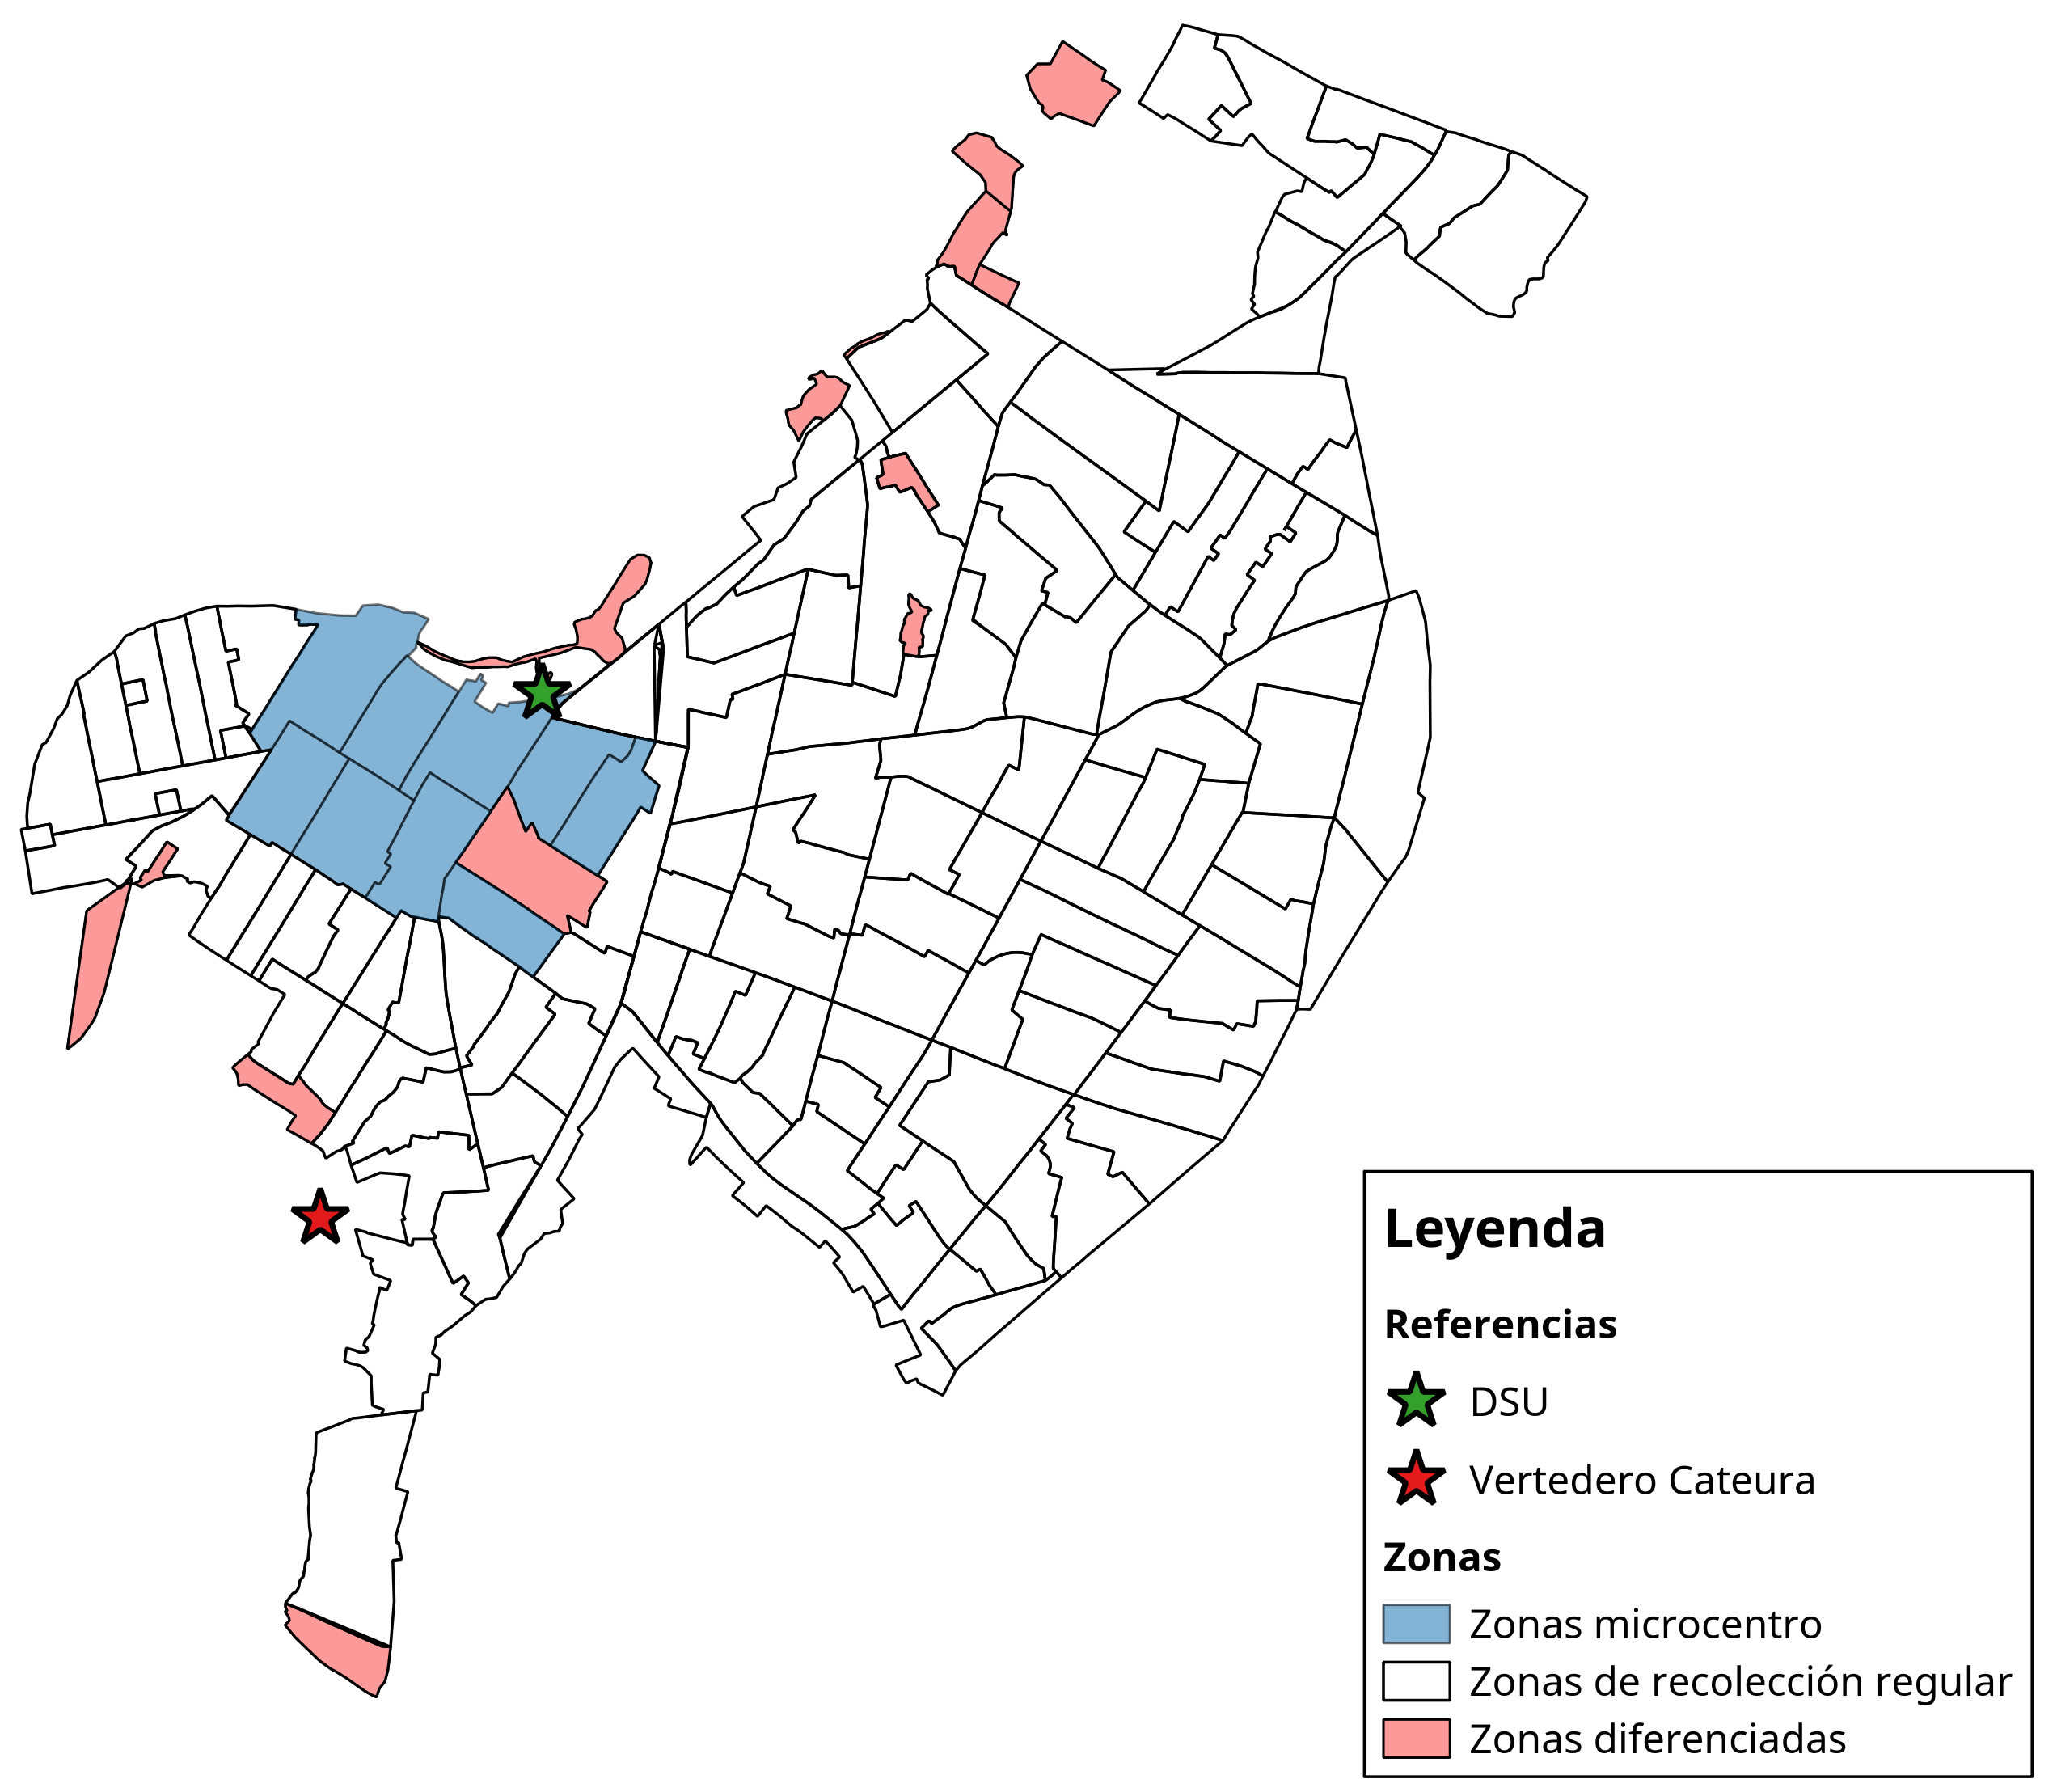
\includegraphics[width=8cm]{Recoleccion-ZONAS_CUADRANTES.png}
    \caption{División de la ciudad en zonas.}
    \label{fig:zonasRecoleccion}
\end{figure}

Los residuos sólidos de grandes generadores son todos aquellos residuos sólidos urbanos comerciales cuyas cantidades requieran una recolección diferenciada, esta recolección no forma parte del procedimiento descrito más arriba y tampoco se incluye en el alcance de este trabajo. Los residuos hospitalarios son recolectados por una empresa tercerizada por el municipio y no son depositados en Cateura.

% En la actualidad, los choferes de los vehículos recolectores de basura de la ciudad de Asunción trazan los caminos a seguir en base a su experiencia, razón por la cual es necesario optimizar el recorrido realizado para la recolección de residuos, reduciendo el costo y el tiempo de cada recorrido. Se propone desarrollar una aplicación que permita gestionar de manera eficiente esos recorridos al poder actualizar el sentido de las calles, inhabilitar calles, agregar restricciones de giro o de continuar el sentido (contramano).

% \begin{itemize}
% \item Se establecen los días y frecuencias de recolección para cada zona.
% \item Un equipo de trabajo cuenta con un chofer y tres recolectores, que es asignado a un vehículo y una zona. El vehículo es identificado por su chapa o por el número de identificación del camión proveído por la DSU. Estos vehículos recolectores son de propiedad de la MDA, en caso de que uno de ellos quede fuera de servicio por algún desperfecto, por lo general, la solución radica en alquilar un recolector para que lo cubra. TODO: la ultima oracion es la que se quito del paper
% \item Se realiza una recogida no selectiva. En la Ordenanza Municipal N$^{\circ}$ 408/14 se establece que los usuarios del servicio ordinario de recolección deberán almacenar sus residuos en el interior de las viviendas o locales correspondientes, en  sitios adecuados, en bolsas perfectamente cerradas, las cuales serán sacadas y colocadas en la acera, solamente en los días señalados, momento antes del horario fijado para el servicio. No se permitirá el acopio o acumulación de los residuos en la vía pública, ya sea directamente sobre las aceras o en canastos elevados en días y horas distintos a los establecidos para el servicio de recolección. TODO: la parte de la ordenanza es la que se omitio en el paper
% \item El vehículo recolector inicia su recorrido cuando parte de la DSU en dirección a su zona. Antes de partir se controla el nivel de combustible y de acuerdo a esto se procede a la carga del mismo, en caso de que fuese necesario. Se entrega al chofer una orden de trabajo del día con la hora de salida. En la Figura \ref{fig:vehiculoRecolectorMDA}, se muestra un vehículo recolector de la MDA.
% \item Luego de haber recogido toda la basura domiciliaria de la zona, el vehículo se dirige al relleno sanitario Cateura para depositar los residuos y de allí vuelve a su punto de partida. Generalmente, el vehículo tiene capacidad suficiente para realizar un solo viaje de su zona a Cateura, pero si no es el caso, debe realizar la cantidad de viajes necesarios hasta recolectar todos los residuos domiciliarios de la zona en cuestión. La carga máxima admitida de un vehículo recolector en circulación por el Departamento de Recolección de la DSU es de 8500 Kg, en caso de que el equipo de trabajo estime, en base a su experiencia, que la cantidad total a recoger de la zona será mayor al permitido, entonces realiza más de un viaje a Cateura.
% \item Una vez que el chofer llega a Cateura, el camión pasa por un pesaje por ejes con báscula y el chofer entrega la orden de trabajo a un fiscalizador que se encuentra en el puesto de pesaje. Un grupo de personas de seguridad se encargan de coordinar la entrada y salida de vehículos, así como de guiar la descarga de lo recolectado. En el lugar se encuentran varios gancheros que ayudan a sacar los residuos del vehículo, los gancheros son personas dedicadas a recuperar, separar o reducir, de los residuos sólidos urbanos, aquellos que posean valor comercial para su reutilización o reciclaje. Una vez que se vacía el vehículo, uno de los encargados guía nuevamente al chofer hacia la salida, en donde el vehículo es pesado de vuelta, calculando así el peso de lo recolectado, que se detalla en la orden de trabajo la cual es devuelta al chofer. En la orden de trabajo también se especifican la hora de entrada y salida del vehículo al relleno sanitario.
% \item Una vez que el equipo de trabajo se encuentra de vuelta en la DSU, el chofer entrega la orden de trabajo al Departamento de Recolección.
% \end{itemize}

%TODO: cambiar por el shape que nos dieron%


% El servicio de recolección domiciliaria se realiza de lunes a sábados, y se divide en tres turnos: mañana, tarde y noche; donde cada turno tiene una duración máxima de 6 horas debido al carácter insalubre de las tareas realizadas por el personal encargado de brindar el servicio.

% En la figura \ref{fig:zonasRecoleccion} un turno se corresponde con un conjunto de zonas, las zonas pintadas en azul oscuro, correspondientes al microcentro de Asunción, tienen un tratamiento diferente a las demás zonas, ya que son las únicas que son atendidas de lunes a viernes, las demás zonas reciben el servicio cada dos días, tres veces por semana. Los residuos en estas zonas son recolectados en el turno noche debido al poco tráfico registrado en esas calles en comparación a cualquier otro turno, de igual manera, las avenidas más importantes de la ciudad también son recolectadas en el turno noche de lunes a viernes, los equipos de trabajo que recogen los residuos a lo largo de estas avenidas les corresponden dos avenidas por noche. Las zonas no pintadas no tienen número, y por ende no son cubiertas por el servicio, sin embargo representan una zona candidata a futuro para la recolección de la basura.

% Los residuos sólidos de grandes generadores son todos aquellos residuos sólidos urbanos comerciales cuyas cantidades requieran una recolección diferenciada, esta recolección no forma parte del procedimiento descrito más arriba y tampoco se incluye en el alcance de este trabajo. Los residuos hospitalarios son recolectados por una empresa tercerizada por el municipio y no son depositados en Cateura.

% La recolección de los residuos de manejo especial y peligrosos no forman parte lo descrito más arriba y tampoco forman parte del alcance de este trabajo.